\chapter{Strategy Extraction}
\label{ch:strategy}

\newcommand{\strategyext}[0]{\textsc{strategyGen}\xspace}
\newcommand{\genstrategy}{\textsc{strategyGen}}
\newcommand{\strategy}[0]{\textsc{strategy}\xspace}
\newcommand{\partition}[0]{\textsc{partition}\xspace}
\newcommand{\ogametree}[0]{\mbox{\sc OppGT}}
\newcommand{\eagametree}[0]{\mbox{\sc AbsGT}'}
\newcommand{\pgametree}[0]{\mbox{\sc Cand}}
\newcommand{\apgametree}[0]{\mbox{\sc AbsSolvedGT}}
\newcommand{\opgametree}[0]{\mbox{\sc Spoiling}}

\newcommand{\opptf}[0]{\textsc{\textoverline{treeFormula}}\xspace}

\newcommand{\clk}[0]{\texttt{clk}}
\newcommand{\curr}[0]{\texttt{curr}}
\newcommand{\err}[0]{\texttt{err}}
\newcommand{\nex}[0]{\texttt{next}}
\newcommand{\inp}[0]{\texttt{in}}

In the previous chapter I introduced an algorithm for solving realisability for bounded safety games. In most applications of synthesis it is desirable to construct a controller strategy rather than merely prove its existence. In this chapter I will introduce a strategy extraction procedure that complements the bounded reachability algorithm. This process takes abstract game trees generated during reachability analysis and, using Craig interpolation, extracts mappings of states to player actions. By using interpolation this step can be done efficiently.

The problem solved in this chapter is related to the extraction of a Skolem function for a QBF. Recall from Chapter~\ref{ch:background} that a Skolem function $f$ provides a mapping from a prefix of universal variables $\hat{y}_0, \hat{y_1}, \ldots, \hat{y_i}$ to existential variables $\hat{x}$ such that when substituting $\hat{x}$ for $f(\hat{y}_0, \hat{y_1}, \ldots, \hat{y_i})$ the QBF is equisatisfiable. A Skolem function for a bounded realisability QBF gives a mapping from a prefix of past environment actions to a controller action, i.e. a strategy for that game round. A strategy for the entire game consists of a Skolem function for every round. We simplify the problem by constructing a single function $\pi$ that maps states and environment actions to controller actions. The game is deterministic, so an assignment to variables in the quantifier prefix corresponds to exactly one state and action pair.  If we guarantee that all successors states reachable by playing according to the strategy in round $k$ have a winning strategy defined by $\pi$ for a game bounded to $k-1$ rounds then this function may be used as a Skolem function in every round of the game. Thus we are able to solve a simpler problem than Skolemisation of the entire QBF by taking advantage of the structure of bounded realisability.

\section{Algorithm}

Recall that a safety game is a tuple $(\cS, \cU, \cC, \delta, s_0)$ where $\cS$ is a set of state variables, $\cU$ a set of environment action variables, $\cC$ a set of controller action variables, $\delta$ defines a transition relation, and $s_0$ is an initial state. A set of states $E$ provides the winning condition, the controller must avoid error states and the environment must reach one. A winning strategy for controller is a function $\pi^c : 2^\cS \times 2^\cU \to 2^\cC$ that avoids error states for the duration of the game. A controller strategy is then a mapping from state and environment-action pairs to controller actions. For convenience we use $\cW = \cS \cup \cU$ to denote the set of boolean variables that serve as input to the function defining a strategy.

In this chapter we will assume that the safety game is realisable and a winning strategy for the controller exists. However, the technique is also easily applied to unrealisable games to extract a spoiling strategy that is winning for the environment. In computing realisability of a safety game the algorithm constructs a \emph{certificate tree}, which is an abstract game tree $T$ such that for a set of states $s$ and game bound $\kappa$, $s \land \opptf(\kappa, \textsc{extend}(T))$ is false. In other words it is a game abstraction for which the environment has no candidate strategy.

We use the certificate tree computed by the game solver as a starting point for strategy generation.  We know that the controller can win the game in $\kappa$ rounds by picking actions from the tree; however we do not yet know which action to choose in which situation.


\subsection{Example}

Figure~\ref{fig:stratExample} introduces the running example for this chapter. It shows a state machine for a game $(\mathcal{S}, \mathcal{U}, \mathcal{C}, \delta, s_0)$ that describes the operation of a simpled clocked flip-flop. For the example we model the clock as part of the game state and assume that it oscillates in every game round. So $\cS = \{ \clk, \curr, \err \}$ are the state variables of the game and contains the clock, the current value of the flip-flop, and an error bit respectively. The environment has a single data bit variable: $\cU = \{ \inp \}$ and the controller has the next value of the flip-flop: $\cC = \{ \nex \}$. The diagram shows $\delta$ as a deterministic finite state automaton with edges labelled by a tuple $(\inp, \nex)$. We use $*$ as a wildcard value to simplify the presentation. The circuit described by the specification allows the environment to save a bit $\inp$ into the flip-flop when the clock has a falling edge ($\clk$ transitions from $1$ to $0$). The controller must correctly set $\nex$ so that $\curr$ always contains the correct data. The initial state, $s_0$, is $(\clk = 0 \land \curr = 0 \land \err = 0)$ and the error set is given by $(\err = 1)$.

\tikzset{
    pil/.style={
        -{Latex[length=3mm]},
        thick
    },
    snode/.style={
        align=center,
        circle,
        draw,
        thick
    }
}

\begin{figure}
    \centering
    \begin{tikzpicture}
        \node [snode]
            (s1){$\clk = 0$ \\ $\curr = 0$ \\ $\err = 0$};
        \node [draw=none,left=of s1] (i){};
        \node [snode,below=1.5cm of s1]
            (s0){$\clk = 1$ \\ $\curr = *$ \\ $\err = 0$};
        \node [snode,right=2.5cm of s0]
            (s3){$\clk = 0$ \\ $\curr = 1$ \\ $\err = 0$};
        \node [snode,accepting,right=2.5cm of s1]
            (err){$\clk = *$ \\ $\curr = *$ \\ $\err = 1$};

        \draw [pil] (i) edge (s1);

        \draw [pil] (s0) edge [bend left] node [left] {$(0, 0)$} (s1);
        \draw [pil] (s1) edge [bend left] node [left] {$(*, 0)$} (s0);

        \draw [pil] (s0) edge [bend left] node [below] {$(1, 1)$} (s3);
        \draw [pil] (s3) edge [bend left] node [below] {$(*, 1)$} (s0);

        \draw [pil] (s1) edge node [above] {$(*, 1)$} (err);
        \draw [pil] (s3) edge node [right] {$(*, 0)$} (err);
        \draw [pil] (s0) edge node [above left=0mm and -3mm] {$(*, \lnot \inp)$} (err);
%%%        \draw [pil] (s1) edge node [below right] {$(*, 0)$} (err);
    \end{tikzpicture}
    \caption{Transition relation of the running example}
    \label{fig:stratExample}
\end{figure}

Algorithm~\ref{alg:strat} shows the pseudocode of the strategy generation algorithm.  The algorithm proceeds in two phases: the first phase (\textsc{genLocalStrats}) computes local strategies in nodes of $T$; the second phase (\textsc{compileStrat}) compiles all local strategies into a winning strategy function.

The \textsc{genLocalStrats} function recursively traverses the certificate tree $T$, starting from the root, computing local strategies in each node.  The main operation of the algorithm, called \textsc{partition}, splits $(T, s_0)$ into $j$ tuples $(T_i, \sigma_i)$, as shown in Figure~\ref{fig:partition}.  Each tree $T_i$ is a copy of a single branch of $T$ and the series $\sigma_1 \ldots \sigma_i$ forms a disjoint partitioning of $s_0$ and environment actions, i.e. $\sigma_i \subseteq s_0 \subseteq 2^{\mathcal{S}} \times 2^{\mathcal{U}}$.  The partitioning is constructed in such a way that the action $c_i$ that labels the root edge of $T_i$ is a winning controller action for states and environment actions in $\sigma_i$.

\begin{figure}[b]
    \centering
    \captionsetup[subfigure]{width=\textwidth,justification=centering}
    \hspace*{\fill}%
    \begin{subfigure}[t]{.4\textwidth}
        \centering
        \begin{minipage}[t][3cm][t]{\textwidth}
        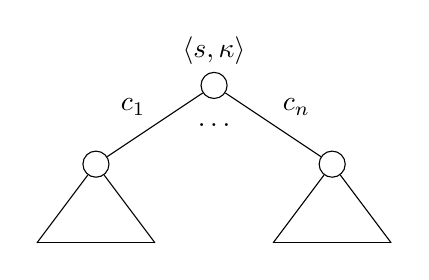
\begin{tikzpicture}[level distance = 10mm,baseline]
            \node [circle,draw] (root){}
                child {node [circle,draw] (left0){}
                    child {node (left1){}
                        edge from parent [draw=none]
                    }
                    child {node (left2){}
                        edge from parent [draw=none]
                    }
                    edge from parent node [above left] {$c_1$}
                }
                child {node [circle] {}
                    edge from parent [draw=none] node [] {$\ldots$}
                }
                child {node [circle,draw] (right0){}
                    child {node (right1){}
                        edge from parent [draw=none]
                    }
                    child {node (right2){}
                        edge from parent [draw=none]
                    }
                    edge from parent node [above right] {$c_n$}
                }
                node [left=4pt] {}
                node [above=4pt] {$\langle s, \kappa \rangle$};

            \draw (left1.center) -- (left2.center);
            \draw (left0) -- (left1.center);
            \draw (left0) -- (left2.center);
            \draw (right1.center) -- (right2.center);
            \draw (right0) -- (right1.center);
            \draw (right0) -- (right2.center);
        \end{tikzpicture}
        \end{minipage}
        \caption{Before}
    \end{subfigure}\hfill%
    \begin{subfigure}[t]{.3\textwidth}
        \centering
        \begin{minipage}[t][3cm][t]{\textwidth}
        \begin{tikzpicture}[level distance = 10mm,baseline]
            \node [circle,draw] (root){}
                child {node [circle,draw] (left0){}
                    child {node (left1){}
                        edge from parent [draw=none]
                    }
                    child {node (left2){}
                        edge from parent [draw=none]
                    }
                    edge from parent node [left] {$c_1$}
                }
                node [above=4pt] {$\langle \sigma_1, \kappa \rangle$};

            \node [draw=none,below right=25pt and 22pt] {$\ldots$};

            \begin{scope}[xshift=60pt]
            \node [circle,draw] (root2){}
                child {node [circle,draw] (right0){}
                    child {node (right1){}
                        edge from parent [draw=none]
                    }
                    child {node (right2){}
                        edge from parent [draw=none]
                    }
                    edge from parent node [right] {$c_n$}
                }
                node [left=4pt] {}
                node [above=4pt] {$\langle \sigma_n, \kappa \rangle$};
            \end{scope}

            \node [below=5pt of left0] {$T_1$};
            \node [below=5pt of right0] {$T_n$};
            \draw (left1.center) -- (left2.center);
            \draw (left0) -- (left1.center);
            \draw (left0) -- (left2.center);
            \draw (right1.center) -- (right2.center);
            \draw (right0) -- (right1.center);
            \draw (right0) -- (right2.center);
        \end{tikzpicture}
        \end{minipage}
        \caption{After}
    \end{subfigure}%
    \hspace*{\fill}
    \caption{Partitioning}
    \label{fig:partition}
\end{figure}

Figure~\ref{fig:algex} illustrates how local strategies are generated from the winning abstract game tree returned by the game solver for our running example.  Figure~\ref{fig:algexa} shows $T$, the certificate tree of height 3 for the game. The algorithm starts at the root of the tree and the initial state $s = (\clk = 0 \land \curr = 0 \land \err = 0)$.  The game tree defines only one winning action in the root node, hence this action is winning in all states of $s$ and against all actions and no partitioning is required. We project $s$ onto the combined set of states and actions, i.e. $\sigma = s(\cW)$, such that $\nex = 0$ is winning for $\sigma$. We now compute the successor set reachable by playing action $\nex = 0$ against $\sigma$: i.e. we compute the set $s' \subseteq 2^{\cS'}$ such that $\exists \cS \exists \cU \exists \cC (\delta(\cS, \cU, \cC, \cS') \land \sigma \land (\nex = 0))$, which evaluates to $s' = (\clk = 1 \land \err = 0)$.

\tikzset{every node/.style={solid}}
\begin{figure}[b]
    \centering
    \captionsetup[subfigure]{width=\textwidth,justification=centering}
    \begin{subfigure}[t]{.5\textwidth}
        \centering
        \begin{minipage}[t][4cm][t]{\textwidth}
        \centering
        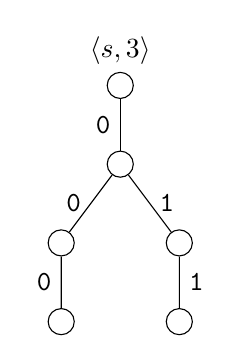
\begin{tikzpicture}[level distance = 10mm,baseline]
            \node [circle,draw] (root){}
                child {node [circle,draw] {}
                    child {node [circle,draw] {}
                        child {node [circle,draw] {}
                            edge from parent node [left] {\texttt{0}}
                        }
                        edge from parent node [left] {\texttt{0}}
                    }
                    child {node [circle,draw] {}
                        child {node [circle,draw] {}
                            edge from parent node [right] {\texttt{1}}
                        }
                        edge from parent node [right] {\texttt{1}}
                    }
                    edge from parent node [left] {\texttt{0}}
                }
                node [above=4pt] {$\langle s, 3 \rangle$};
        \end{tikzpicture}
        \end{minipage}
        \caption{$T$}
        \label{fig:algexa}
    \end{subfigure}%
    \begin{subfigure}[t]{.5\textwidth}
        \centering
        \begin{minipage}[t][4cm][t]{\textwidth}
        \centering
        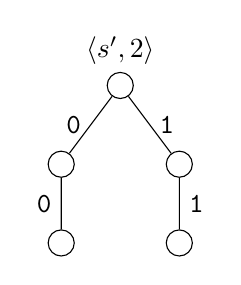
\begin{tikzpicture}[level distance = 10mm,baseline]
            \node [circle,draw] (root){}
                child {node [circle,draw] {}
                    child {node [circle,draw] {}
                        edge from parent node [left] {\texttt{0}}
                    }
                    edge from parent node [left] {\texttt{0}}
                }
                child {node [circle,draw] {}
                    child {node [circle,draw] {}
                        edge from parent node [right] {\texttt{1}}
                    }
                    edge from parent node [right] {\texttt{1}}
                }
                node [above=4pt] {$\langle s', 2 \rangle$};
        \end{tikzpicture}
        \end{minipage}
        \caption{$T'$}
        \label{fig:algexb}
    \end{subfigure}
    \begin{subfigure}[t]{.5\textwidth}
        \centering
        \begin{minipage}[t][3cm][t]{\textwidth}
        \centering
        \begin{tikzpicture}[level distance = 10mm,baseline]
            \node [circle,draw] (root1){}
                child {node [circle,draw] {}
                    child {node [circle,draw] {}
                        edge from parent node [left] {\texttt{0}}
                    }
                    edge from parent node [left] {\texttt{0}}
                };
            \node [above=4pt of root1] {$\langle \sigma_1', 2 \rangle$};

            \node [circle,draw,right=2cm] (root2){}
                child {node [circle,draw] {}
                    child {node [circle,draw] {}
                        edge from parent node [right] {\texttt{1}}
                    }
                    edge from parent node [right] {\texttt{1}}
                };
            \node [above=4pt of root2] {$\langle \sigma_1', 2 \rangle$};
        \end{tikzpicture}
        \end{minipage}
        \caption{Partitioning of $T'$ into $T_1'$ and $T_2'$}
        \label{fig:algexc}
    \end{subfigure}%
    \begin{subfigure}[t]{.5\textwidth}
        \centering
        \begin{minipage}[t][3cm][t]{\textwidth}
        \centering
        \begin{tikzpicture}[level distance = 10mm,baseline]
            \node [circle,draw] (root1){}
                child {node [circle,draw] {}
                    edge from parent node [left] {\texttt{0}}
                };
            \node [above=4pt of root1] {$\langle s_1'', 1 \rangle$};

            \node [circle,draw,right=2cm] (root2){}
                child {node [circle,draw] {}
                    edge from parent node [right] {\texttt{1}}
                };
            \node [above=4pt of root2] {$\langle s_2'', 1 \rangle$};
        \end{tikzpicture}
        \end{minipage}
        \caption{$T_1''$ and $T_2''$}
        \label{fig:algexd}
    \end{subfigure}
    \caption{Operation of the strategy extraction algorithm on the example}
    \label{fig:algex}
\end{figure}

Next, we descend down the tree and consider subtree $T'$ and its initial set $s'$ (Figure~\ref{fig:algexb}).  We partition $\sigma' = s'(\cW)$ into gubsets $\sigma_1' = (\clk = 1 \land \err = 0 \land \inp = 0)$ and $\sigma_2' = (\clk = 1 \land \err = 0 \land \inp = 1)$ that are winning for the left and right subtrees of $T'$ respectively, i.e., from $(\clk = 1 \land \err = 0)$ the controller must play action $\nex = 0$ when the environment plays $\inp = 0$, and $\nex = 1$ for $\inp = 1$.  Consider the resulting subtrees $T'_1$ and $T'_2$ with initial sets $\sigma'_1$ and $\sigma'_2$ (Figure~\ref{fig:algexc}).  We compute successor states as before: $s''_1 = (\clk = 1 \land \curr = 0 \land \err = 0)$ and $s''_2 = (\clk = 1 \land \curr = 1 \land \err = 0)$, with corresponding subtrees $T''_1$ and $T''_2$ (Figure~\ref{fig:algexd}).  Both subtrees have one branch; hence the actions in those branches $\nex = 0$ and $\nex = 1$ are winning for $\sigma''_1 = s''_1(\cW)$ and $\sigma''_2 = s''_2(\cW)$ respectively.

The algorithm returns the set of tuples $(\sigma, c, k)$.  Each tuple represents a fragment of the strategy in some tree node, where $\sigma \subseteq 2^{\cW}$ is the winning set in this node, $c \in 2^\cC$ is the controller action to play in this set, and $k$ is the distance from the node to the bottom of the tree.

Putting together fragments of the winning strategy computed above, we obtain the partial strategy shown below for this example. A complete strategy can be constructed by asigning arbitrary actions to all other states as they are known to be unreachable by playing the partial strategy.
\begin{align*}
    \pi(\clk = 0 \land \curr = 0 \land \err = 0) &= (\nex = 0) \\
    \pi(\clk = 1 \land \err = 0 \land \inp = 0) &= (\nex = 0) \\
    \pi(\clk = 1 \land \err = 0 \land \inp = 1) &= (\nex = 1) \\
    \pi(\clk = 0 \land \curr = 1 \land \err = 0) &= (\nex = 1)
\end{align*}



%%%\subsection{Local Strategies}

%%%Algorithm~\ref{alg:strat} shows the pseudocode of the strategy generation algorithm.  The algorithm proceeds in two phases: the first phase (\textsc{genLocalStrats}) computes local strategies in nodes of $T$; the second phase (\textsc{compileStrat}) compiles all local strategies into a winning strategy function.

%%%The \textsc{genLocalStrats} function recursively traverses the certificate tree $T$, starting from the root, computing local strategies in each node.  The main operation of the algorithm, called \textsc{partition}, splits $(T, s, \top)$ into $j$ tuples $(T_i, s_i, u_i)$, as shown in Figure~\ref{fig:partition}.  Each tree $T_i$ is a copy of a single branch of $T$.  The partitioning is constructed in such a way that the action $c_i$ that labels the root edge of $T_i$ is a winning controller action in $s_i$ against environment action $u_i$.

%%%Consider each tuple $(T_i, s_i, u_i)$ (lines~\ref{alg:strat:for}-\ref{alg:strat:endfor}). We descend down the tree and compute the controller strategy in the child subtree $T_i'$ of $T_i$ (right-hand side of Figure~\ref{fig:partition}).  To do so, we first compute the set of $c_i$-successors of $(s_i, u_i)$: More precisely, we compute an overapproximation $\mathcal{I} \supseteq \{ s_i' \mid \delta(s_i, u_i, c_i, s_i') \}$, such that $T_i'$ is a certificate tree for $\mathcal{I}$.  Such an overapproximation is returned by the \textsc{next} function in line~\ref{alg:strat:next}.  We can now recursively invoke the strategy generation function to compute a winning strategy for the subtree $T_i'$ from $\mathcal{I}$ (line~\ref{alg:strat:rec}).

\begin{algorithm}
   \caption{Computing a winning strategy}\label{alg:strat}
   \begin{algorithmic}[1]
        \Function{GenStrategy}{$T$, $k$, $s$}
            \State $Strat \gets \Call{GenLocalStrats}{T, k, s}$
            \State \Return{$\Call{CompileStrat}{Strat}$}
        \EndFunction
        \Statex

        \Function{GenLocalStrats}{$T$, $k$, $s$}
            \State $[(e_1, n_1),\ldots,(e_j, n_j)] \gets \Call{succ}{T}$
            \State $[(T_1,\sigma_1),\ldots,(T_j, \sigma_j)] \gets \Call{partition}{T, k, s(\cS_T) \land \neg E(\cS_T)}$
            \State $Strat \gets \{(\sigma_i, \Call{action}{e_i}, \Call{height}{k, T}) \mid i \in[1,\ldots,j]\}$\label{alg:strat:strati}
            \For{$i = 1$ to $j$}\label{alg:strat:for}
            \State $(T_i', s_i') \gets \Call{next}{T_i, k, \sigma_i}$\label{alg:strat:next}
                \State $Strat_i \gets \Call{GenLocalStrats}{T_i', k-1, s_i'}$\label{alg:strat:rec}
                \State $Strat \gets Strat \cup Strat_i$
            \EndFor\label{alg:strat:endfor}
            \State \Return{$Strat$} \label{alg:strat:return}
        \EndFunction
    \end{algorithmic}
\end{algorithm}


\subsection{Partitioning game trees}

The algorithm described so far involves two potentially costly operations: winning set partitioning and successor set computation.  If implemented na\"ively in a SAT based approach these operations can lead to unacceptable performance. Both operations must return sets and enumerating sets of satisfying assignments with SAT is inefficient. The key insight behind our solution is that both operations can be efficiently approximated from the proof of unsatisfiability of the formula $s \land \opptf(k, T)$, with the help of interpolation, as described below.  The resulting approximations are sound, i.e., preserve the correctness of the resulting strategy.

The \textsc{partition} function (Algorithm~\ref{alg:strat:partition}) computes a local strategy in the root of an abstract game tree.  It takes a tuple $(T, k, s)$, such that $T$ is a certificate tree of height $k$ for states $s$ and partitions $\sigma = s(\cW)$ into subsets $\sigma_i$ such that the controller can win a game of $k$ rounds in the states and against the environment actions contained in $\sigma_i$ by choosing action $c_i$.

\begin{algorithm}[t]
   \caption{Partitioning winning states}\label{alg:strat:partition}
   \begin{algorithmic}[1]
        \Function{partition}{$T$, $k$, $s$}
        \State $\hat{\sigma} \gets s(\cW)$
        \State $\hat{T} \gets T$
        \For{$i = 1$ to $j$}
        \State $(T_i, \tilde{T}) \gets \Call{split}{\hat{T}}$\label{alg:partition:split}
            \State $A \gets \sigma \land \Call{\opptf}{k, \tilde{T}} $ \label{alg:strat:partition:Bi}
            \State $B \gets \Call{\opptf}{k, T_i} $ \label{alg:strat:partition:Ai}
            \State $\mathcal{I} \gets \Call{interpolate}{A, B}$\label{alg:partition:I}
            \State $\sigma_i \gets \mathcal{I}(\cW_T)$\label{alg:partition:Ii}
            \State $\hat{\sigma} \gets \hat{\sigma} \land \neg \sigma_i$
            \State $\hat{T} \gets \tilde{T}$\label{alg:partition:upd}
        \EndFor
        \State \Return{$[(T_1, \sigma_1),\ldots, (T_j, \sigma_j)]$} \label{alg:strat:partition:return}
        \EndFunction
    \end{algorithmic}
\end{algorithm}

At every iteration, the algorithm splits the tree into the leftmost branch $T_i$ and the remaining tree (Figure~\ref{fig:split}).  It then computes $\sigma_i$ where the controller wins by following the branch $T_i$, and removes $\sigma_i$ from the current $\hat{\sigma}$.  At the next iteration it considers the leftover tree $\tilde{T}$ and state-action set $\hat{\sigma}$.

\begin{figure}
    \centering
    \begin{tikzpicture}[level distance = 12mm,baseline]
        \node [circle,draw] (root){}
            child {node [circle,draw] (left0){}
                child {node (left1){}
                    edge from parent [draw=none]
                }
                child {node (left2){}
                    edge from parent [draw=none]
                }
                edge from parent node [below left=-1mm and 3mm] {$c_i$}
            }
            child {node [circle,draw,right=8mm] (leftb0){}
                child {node (leftb1){}
                    edge from parent [draw=none]
                }
                child {node (leftb2){}
                    edge from parent [draw=none]
                }
                edge from parent node [below right=-1mm and 2mm] {$c_{i+1}$}
            }
            child {node [circle,draw,right=11mm] (leftc0){}
                child {node (leftc1){}
                    edge from parent [draw=none]
                }
                child {node (leftc2){}
                    edge from parent [draw=none]
                }
                edge from parent node [below right=-1mm and 5mm] {$c_{j}$}
            }
            node [above=4pt] {$(\hat{T}, \hat{\sigma})$};


        \node [draw,
            dash pattern=on 2pt off 2pt,
            minimum width=6.5cm,
            minimum height=4cm,
            below right=-10mm and -27mm
            ] {};
        \node [above=8mm of root] (startline) {};
        \node [below=29mm of root] (endline) {};
        \draw [dash pattern=on 2pt off 2pt] (startline) -- (endline);

        \node [below=5pt of left0] {$T_i$};
        \node [below=5pt of leftb0] {$T_{i+1}$};
        \node [below=5pt of leftc0] {$T_j$};
        \draw (left1.center) -- (left2.center);
        \draw (left0) -- (left1.center);
        \draw (left0) -- (left2.center);
        \draw (leftb1.center) -- (leftb2.center);
        \draw (leftb0) -- (leftb1.center);
        \draw (leftb0) -- (leftb2.center);
        \draw (leftc1.center) -- (leftc2.center);
        \draw (leftc0) -- (leftc1.center);
        \draw (leftc0) -- (leftc2.center);
        \node [right=4mm of leftb0] {$\ldots$};
        \node [above=6mm of left0] {$(T_i, \sigma_i)$};
        \node [above=6mm of leftc0] {$(\tilde{T}, \hat{\sigma} \setminus \sigma_i)$};
    \end{tikzpicture}
    \caption{Splitting of $T$ in the \textsc{Partition} function.\label{fig:split}}
\end{figure}

The algorithm maintains the invariant that $\hat{T}$ is a certificate tree of height $k$ for $\hat{\sigma}$, and hence $\hat{\sigma} \land \opptf(k, \hat{T})$ is unsatisfiable.  We decompose this formula into two conjuncts $A \land B$ such that $A$ and $B$ only share state and action variables $\cW_T$ in the root node of $T$ and that the interpolant $\mathcal{I}$ of $A$ and $B$ consists of states and environment actions for which the controller can win by following the $T_i$ subtree.  Hence $\mathcal{I}(\cW_T)$ gives us the desired set $\sigma_i$.  

Informally, $A$ is a partial expansion of the game formula induced by $\tilde{T}$.  It is satisfiable iff there exists a spoiling environment strategy from $\hat{\sigma}$ against abstract game tree $\tilde{T}$.  $B$ is a partial expansion of the game induced by $T_i$.  It is satisfiable iff there exists a spoiling environment strategy against $T_i$.  Both $A$ and $B$ can be satisfiable individually, but because $T$ is a certificate tree their conjunction is unsatisfiable.

The interpolant $\mathcal{I}$ of $A$ and $B$ implies $\neg B$, i.e., for any state and environment action in $\mathcal{I}$, $c_i$ is a winning move.  $\mathcal{I}$ is also implied by $A$, i.e., it contains all states and environment actions in $\hat{\sigma}$ for which the controller cannot win by picking moves from $\tilde{T}$ as a subset.  Equivalently, for any state and action in $\hat{\sigma} \land \neg \mathcal{I}(\cW_T)$, the controller \emph{can} win by following $\tilde{T}$, i.e., $\tilde{T}$ is a certificate tree for $\hat{\sigma} \land \neg \mathcal{I}(\cW_T)$, and we can apply the decomposition again to $\tilde{T}$ at the next iteration.


\makeatletter
\newcommand{\pushright}[1]{\ifmeasuring@#1\else\omit\hfill$\displaystyle#1$\fi\ignorespaces}
\makeatother

We prove useful properties of the $\partition$ function. We begin with the proposition that $A$ and $B$ imply a decomposition of $\hat{\sigma} \land \opptf(k, \hat{T})$. 
\begin{proposition}\label{prop:aandb}
    $A\land B \implies \hat{\sigma} \land \opptf(k, \hat{T})$.
\end{proposition}
\begin{proof}
    \begin{align*}
        A \land B ={}& (\hat{\sigma} \land \opptf(k, \tilde{T})) \land \opptf(k, T_i) \\
        A \land B ={}& \hat{\sigma} \land \bigg( E({\mathcal{S}_{\tilde{T}})} \lor \\
                     & \pushright{ \bigvee_{\langle e, n \rangle \in \textsc{succ}(\tilde{T})} \delta({\mathcal{S}_{\tilde{T}}}, {\mathcal{U}_{\tilde{T}}}, {\mathcal{C}_{\tilde{T}}}, {\mathcal{S}_n}) \land \textsc{action}(e) \land \opptf(k, n) \bigg)} \\
                     & \pushright{\land \bigg( E({\mathcal{S}_{T_i}}) \lor (\delta({\mathcal{S}_{T_i}}, {\mathcal{U}_{T_i}}, {\mathcal{C}_{T_i}}, {\mathcal{S}_{n_i}}) \land \textsc{action}(e_i) \land \opptf(k, n_i)) \bigg)} \\
        \implies{}& \hat{\sigma} \land \bigg( E({\mathcal{S}_{\hat{T}}}) \lor \\
                  & \pushright{  \bigvee_{\langle e, n \rangle \in \textsc{succ}(\hat{T})} \delta({\mathcal{S}_{\hat{T}}}, {\mathcal{U}_{\hat{T}}}, {\mathcal{C}_{\hat{T}}}, {\mathcal{S}_n}) \land \textsc{action}(e) \land \opptf(k, n) \bigg)} \\
        ={}& \hat{\sigma} \land \opptf(k, \hat{T})
    \end{align*}
\end{proof}

\begin{proposition}
    The following invariant is maintained throughout the execution of \textsc{partition}: $\hat{T}$ is a certificate tree of height $k$ for $\hat{\sigma}$.
\end{proposition}
\begin{proof}
    We prove by induction. It is a precondition of the function that $T$ is a certificate tree for $s$, thus the invariant holds for the initial values $\hat{T} = T$ and $\hat{\sigma} = s(\cW)$.  By the induction hypothesis $(\hat{\sigma} \land \opptf(k, \hat{T}))$ is unsatisfiable, so by Proposition~\ref{prop:aandb} $(A \land B)$ must also be unsatisfiable.  Hence the interpolation operation in line~\ref{alg:partition:I} is well defined.  By the properties of interpolants, $(A \implies \mathcal{I})$, hence $(\neg \mathcal{I} \implies \neg A)$ or equivalently $(\neg\mathcal{I} \implies \neg (\hat{\sigma} \land \opptf(k, \tilde{T}))$.

    After $\hat{T}$ and $\hat{\sigma}$ are updated in line~\ref{alg:partition:upd}, their new values $\hat{T}'$ and $\hat{\sigma}'$ satisfy the following equalities: \begin{align*}
        \hat{\sigma}' \land \opptf(k, \hat{T}') ={}& \hat{\sigma} \land \opptf(k, \tilde{T}) \land \neg\mathcal{I} \\
        ={}& \neg\mathcal{I} \land \hat{\sigma} \land \opptf(k, \tilde{T}) \\
        \implies{}& \neg (\hat{\sigma} \land \opptf(k, \tilde{T})) \\
                  & \pushright{\land \hat{\sigma} \land \opptf(k, \tilde{T})} \\
        ={}& \bot
\end{align*} and hence the invariant is maintained.
\end{proof}

\begin{proposition}\label{prop:partition}
    Let $T$ be a certificate tree for $s$ and let $s \land \lnot E(\cS_T) = \bot$. Then $[(T_1, \sigma_1),\ldots,(T_j, \sigma_j)] = \textsc{partition}(T, s)$ is a local winning strategy in the root of $T$, i.e., the following properties hold:
    \begin{enumerate}
        \item $\sigma_1 ,\ldots, \sigma_j$ is a partitioning of
            $s(\cW)$: $$s(\cW) = \bigvee \sigma_i \text{ and } \forall i, k. (i \neq k) \implies (\sigma_i \land \sigma_k = \bot).$$
        \item $T_i$ is a certificate tree of height $k$ for $\sigma_i$.
    \end{enumerate}
\end{proposition}
\begin{proof}
    At every iteration of the algorithm, we partition $\hat{\sigma}$ into $\sigma_i = \mathcal{I}(\cW_T) \land \hat{\sigma}$ and $\hat{\sigma} \land \neg\mathcal{I}(\cW_T)$. Hence, by construction, no $\sigma_i$ overlaps with any $\sigma_k$.

    At the final iteration of the algorithm, the tree $\tilde{T}$ consists of a single root node without outgoing branches.  Hence, $A = \hat{\sigma} \land \opptf(k, \tilde{T}) = \hat{\sigma} \land \neg E(\cS_{\tilde{T}}) = \hat{\sigma}$.  Since $(A \implies \mathcal{I})$, we get $(\hat{\sigma} \implies \mathcal{I})$ and therefore $\mathcal{I} \land \hat{\sigma} = \hat{\sigma}$, i.e., all states and actions in $\hat{\sigma}$ are included in the final set $\sigma_j$ and hence the partitioning completely covers the set $s(\cW)$: $s=\bigvee \sigma_i$.

    We prove the second statement of the proposition.  The set $\sigma_i$ is computed as $\mathcal{I}(\cW_T) \land \hat{\sigma}$ at the $i$th iteration of the algorithm (line~\ref{alg:partition:Ii}).
    Thus, $$\sigma_i \land \opptf(k, T_i) = \mathcal{I}(\cW_T) \land \hat{\sigma} \land \opptf(k, T_i)$$ By the properties of interpolants, $$\mathcal{I} \land B = \mathcal{I}(\cW_T) \land \opptf(k, T_i) = \bot.$$  Hence $\sigma_i \land \opptf(k, T_i) = \bot$, i.e. $T_i$ is a certificate tree for $\sigma_i$.
\end{proof}

\subsection{Determine an action}

The \textsc{next} function (Algorithm~\ref{alg:next}) takes a set $\sigma$ and its certificate tree $T$ of height $k$, such that there is exactly one outgoing edge, labelled $c$, from the root node of $T$.  $T$ has a sole child subtree $T'$ with root node $n$.  The function computes an overapproximation $s'$ of the $c$-successors of $\sigma$, such that $s'$ is winning for the controller and $T'$ is a certificate tree of height $k-1$ for $s'$.

\begin{algorithm}
   \caption{Successor set}\label{alg:next}
   \begin{algorithmic}[1]
        \Function{next}{$T, k, \sigma$}
        \State $[(e, n)] \gets \Call{succ}{T}$ \Comment{$T$ has a single successor}
            \State $A \gets \sigma \land \delta(\cS_T, \cU_T, \cC_T, \cS_n) \land \Call{action}{e}$\label{alg:strat:partition:Ai}
            \State $B \gets \opptf(k, n) $\label{alg:strat:partition:Bi}
            \State $\mathcal{I} \gets \Call{interpolate}{A, B}$ \label{alg:strat:partition:I}
            \State \Return{$(n, \mathcal{I}(\mathcal{S}_{n}))$} \label{alg:strat:partition:return}
        \EndFunction
    \end{algorithmic}
\end{algorithm}

Once again, we decompose the unsatisfiable formula $\sigma \land \opptf(k, T)$ into two conjuncts $A$ and $B$.  $A$ encodes one round of the game from the set $\sigma$, where the controller plays action $c$.  $B = \opptf(k, T')$ is a partial $\forall$-expansion of the game induced by $T'$.  $A$ and $B$ only share state variables $\cS_n$ (where $n$ is the root node of $T'$ and single successor node of $T$) and their interpolant gives the approximation we are looking for.

\begin{proposition}\label{prop:next}
    Let $T$ be a certificate tree for $\sigma$ with a single outgoing edge, labelled $c$ in its root node, and let $(T',\mathcal{I})
    = \textsc{next}(T,\sigma)$.
    Then:
    \begin{enumerate}
        \item $\mathcal{I}$ is an overapproximation of the $c$-successors of $\sigma$, i.e., $\mathcal{I} \supseteq s'$ where $$s' = \exists \cS \exists \cU \exists \cC (\delta(\cS, \cU, \cC, \cS') \land \sigma \land c)$$
        \item $T'$ is a certificate tree of length $k-1$ for $s'$
    \end{enumerate}
\end{proposition}
\begin{proof}
    The $c$-successor set $s'$ of $\sigma$ is defined by $\exists \cS \exists \cU (\delta(\cS, \cU, \cC, \cS') \land \sigma \land c)$. The matrix of this formula is exactly formula $A$.  Hence the successor set is given by $s' = \exists \cS \exists \cU (A)$.  Since $(A \implies \mathcal{I})$, $s' \implies \exists \cS \exists \cU (\mathcal{I})$.  Since $\mathcal{I}$ is defined over state variables in the root of $T'$ only, the quantifiers can be removed: $s' \implies \mathcal{I}$ or, in the relational form, $\mathcal{I} \supseteq s'$.
    
    We prove the second property by the construction of the interpolant: $(\mathcal{I} \land \opptf(k, T')) = (\mathcal{I} \land B) = \bot$.
\end{proof}

\subsection{Compiling the strategy}

Finally, we describe how local strategies computed by \textsc{genLocalStrats} are combined into a winning strategy for the game.  This requires some care, as individual partial strategies can be defined over overlapping sets of states.  We want the resulting strategy function to be deterministic; therefore for each partial strategy we only add new states not yet covered by the computed combined strategy.  Function \textsc{compileStrats} (Algorithm~\ref{alg:compile}) achieves this by keeping track of all states $W$ already added to the strategy.  For every new tuple $(w, a, k)$, it restricts the set $w$ to $\neg W$, which guarantees that no state action pair can be added to the strategy twice.  

\begin{algorithm}[t]
   \caption{Compiling the  winning strategy}\label{alg:compile}
   \begin{algorithmic}[1]
        \Function{CompileStrat}{$Strat$}
            \State $\pi \gets \bot,~~W \gets \bot$
            \For{$(w, c, k) \in Strat$} \Comment{Sorted by descending $k$}
            \State $\pi \gets \pi \lor (w \land \neg W \land c)$
                \State $W \gets W \lor w$
            \EndFor
            \State \Return $\pi$
        \EndFunction
    \end{algorithmic}
\end{algorithm}

\begin{theorem}[Correctness of the algorithm]\label{th:stratCorrectness}
Let abstract game tree $T$ of height $\kappa$ be a certificate tree for the set $s_0$, let $\pi$ be a partial function returned by the strategy generation algorithm, $\pi=\textsc{genStrategy}(T,s_0)$, and let $\pi'$ be an arbitrary extension of $\pi$ to a complete function.  Then $\pi'$ is a winning controller strategy for the bounded game of length $\kappa$ with initial state $s_0$.
\end{theorem}
\begin{proof}
    $\textsc{genStrategy}$ generates a strategy $\pi$ from the set of tuples $Strat$ returned by $\textsc{genLocalStrats}$. Each tuple $(w, c, k)$ in $Strat$ is generated by \textsc{partition} and, according to Proposition~\ref{prop:partition}, $c$ is a winning controller move from $w$ for a game of length $k$. By Proposition~\ref{prop:next}, all possible $c$-successors of $w$ are covered by subsequent iterations of \textsc{partition} and therefore has some tuple $(w', c', k-1)$ in $Strat$. By constructing $\pi = \textsc{genStrategy}$ from $Strat$ in the order of highest $k$ to lowest, we ensure that any mapping defined by $\pi$ for $w'$ is from a tuple with height $\geq k-1$ and so has a strategy that is winning for the controller for a game of $k-1$ rounds or more.  
    
    Therefore $\pi$ defines a controller action for every state reachable from $s_0$ by playing the strategy. Any extension of $\pi$ to a complete function that maps unreachable states to an arbitrary controller action must then be a winning strategy since the controller is guaranteed to stay within the safe region $W$ by playing $\pi$.
\end{proof}

\section{Optimisations}

\subsection{Strategy extraction with learning}

In Section~\ref{sec:boundedLearning} I described an optimisation to bounded realisability in which computational learning is used to exclude known losing states from the search tree. If this optimisation is enable then the final certificate tree returned by the realisability algorithm will assume the absence of those states. In this case we need to adjust the way that strategy extraction is done so that the generated strategy includes winning actions for excluded states. 

The modification is simple: partial strategies are extracted online during the realisability check. Recall that a set of states $b$ is learned to be losing for the environment for height $k$ when $b \land \opptf(k, T)$ is unsatisfiable for some subtree $T$. In other words, $T$ is a certificate tree for $b$. Algorithm~\ref{alg:stratLearning} shows \textsc{learn} with an additional call to \textsc{genLocalStrats} in line~\ref{line:onlineLocalStrats}.  We use \textsc{genLocalStrats} to record a set of partial strategies, $Strats$, one for each learned state. On termination of the bounded realisability algorithm the entire set $Strats$ is combined into a winning partial strategy with \textsc{compileStrat}.

\begin{algorithm}
    \caption{Learning with online strategy extraction}
    \label{alg:stratLearning}
    \begin{algorithmic}
        \Function{learn}{$p, s, k, T, f$}
            \State $ \hat{s} \gets s$
            \For{$s \in \cS$}
            \State $sol \gets \Call{SATWithAssumptions}{\hat{s} \setminus \{ s \}, f}$
                \If{$sol = \texttt{NULL}$}
                    \State $\hat{s} \gets \hat{s} \setminus \{ s \}$
                \EndIf
            \EndFor
            \If{$p = \texttt{cont}$}
                \State $B^c \gets B^c \lor \hat{s}$
            \Else
                \State $Strats \gets Strats \cup \Call{genLocalStrats}{T, k, \hat{s}}$ \label{line:onlineLocalStrats}
                \For{$i \in [0,\ldots,k]$}
                    \State $B^e[i] \gets B^e[i] \lor \hat{s}$
                \EndFor
            \EndIf
        \EndFunction
    \end{algorithmic}
\end{algorithm}

Algorithm~\ref{alg:stratTreeFml} (reproduced from the previous chapter) shows how an opponent tree formula is constructed with respect to an indexed array of sets of learned states $B^e$. At each index $k$ of the array is a set of states for which the environment is known to lose a game of $k$ rounds. $B^e$ conceptually consists of pairs of state sets and tree heights $(b_i, k_i)$ for which $\textsc{findCandidate}(\textsc{env}, b_i, k_i, T_i)$ returned false for some abstract game tree $T_i$, i.e. $T_i$ is a certificate tree for $(b_i, k_i)$.

\begin{algorithm}
    \caption{Opponent tree formula with state learning}
    \label{alg:stratTreeFml}
    \begin{algorithmic}[1]
        \Function{\textoverline{treeFormula}}{$k, T$}
        \If{$\Call{height}{k, T} = 0$}
        \State \Return{\Call{E}{$\cS_{T}$}}
        \Else
        \State \Return{\Call{$B^e$[\Call{height}{$k,t$}]}{$\cS_{T}$} $\lor$ \\
        $$\bigvee_{\langle e, n \rangle \in \Call{succ}{T}}(\Call{$\delta$}{\cS_T, \cU_T, \cC_e, \cS_n} \land \cC_e = \Call{action}{e} \land \Call{\textoverline{treeFormula}}{k, n})$$ }
        \EndIf
        \EndFunction
    \end{algorithmic}
\end{algorithm}

\begin{theorem}
    Let $G$ be a bounded safety game that is realisable with respect to an error set $E$ and a bound $k$. Let $Strats$ be a set of partial strategies generated during $\textsc{solveAbstract}$, then $\pi = \textsc{compileStrat}(Strats)$ is a winning partial controller strategy for $G$.
\end{theorem}
\begin{proof}
    We prove correctness inductively. At the first online call to \textsc{genLocalStrats}, $B^e$ is empty and by Theorem~\ref{th:stratCorrectness} $Strat_0$ is a partial strategy for a state-round pair $(b_0, k_0)$. $Strat_0$ is added to $Strats$.
    
    In subsequent calls all interpolants are constructed such that $B^e$ is excluded from the game. So, $Strat_{j+1}$ is a partial strategy for a game beginning at $b_{j+1}$ and of length $k_{j+1}$ where every state-round pair $(b_0, k_0), \ldots, (b_k, k_j)$ is assumed unreachable. As in Theorem~\ref{th:stratCorrectness}, all tuples $(w, c, k)$ in $Strat_{j+1}$ are such that $c$ is a winning controller action from $w$ for a game of length $k$ if all $(b_0, k_0), \ldots, (b_k, k_j)$ is assumed unreachable. Likewise, every $c$-successor of $w$ is either covered by $Strat_{j+1}$ or is contained in $(b_0, k_0), \ldots, (b_k, k_j)$.

    Under the inductive hypothesis, $Strats = Strat_0 \cup \ldots \cup Strat_j$ contains winning partial strategies for every $(b_0, k_0), \ldots, (b_j, k_j)$. Thus every state assumed unreachable at the $j+1$ iteration has a winning partial strategy in $Strat_0 \cup \ldots \cup Strat_j$ and so $Strat_0 \cup \ldots \cup Strat_{j+1}$ contains winning partial strategies for all $(b_0, k_0), \ldots, (b_{j+1}, k_{j+1})$.

    Thus, $Strats$ contains winning partial strategies for every state in $B^e$.  \textsc{solveAbstract} terminates when it discovers a certificate tree for the initial state $s_0$. As with all certificate trees generated during execution the algorithm learns from the tree via a call to \textsc{learn}. Thus, at termination $s_0 \in B^e[k]$ and $Strats$ contains a winning partial strategy from $s_0$. Therefore $\pi = \textsc{compileStrat}(Strats)$ is a winning partial controller strategy for the game.
\end{proof}

\subsection{Ensuring compact interpolants}

The implementation of strategy extraction (described in further detail in Chapter~\ref{ch:evaluation}) also contains a small optimisation the ensures that the size of the formulas used in the algorithm do not grow too large. Strategy extraction generates many CNF formulas that are used to construct interpolants. Those formulas also contain interpolants themselves, which are arbitrary formulas that must first be converted to CNF. The usual Tseitin transformation converts a formula to CNF by introducing variables and potentially increases the time taken to determine (un)satisfiability and construct a new interpolant. Fortunately, the interpolants generated by the algorithm are usually not large. This allows us to optimise the implementation by constructing a BDD from each interpolant and using the BDD to efficiently enumerate cubes, which may have a smaller CNF representation. 

BDD sweeping is used to reduce the size of formulas by carefully constructing BDDs from subformulas to deduplicate equivalent parts of the formula~\cite{Kuehlmann97}. The sweep is done carefully so that no one BDD grows too large. The optimisation described here can be seen as a simplistic version of BDD sweeping in which the knowledge that the total formula is small is used to avoid the need for careful BDD construction.

\section{Related work}

All existing strategy extraction algorithms for games were developed for use with game solvers based on winning set compilation~\cite{Bloem14}.  Such a solver generates a sequence of expanding state sets for which the game is safe for $1,2,\ldots$ steps.  The task of the strategy extraction algorithm is to compute a function that in every winning state chooses a single move that forces the game back into a safe state.  In contrast, our strategy generation algorithm does not require the game solver to compile winning regions, but instead uses abstract game trees.

Another line of related work is strategy extraction algorithms for QBF used in QBF certification. QBF strategy extraction methods are specific to the underlying proof system used by the QBF search algorithm~\cite{Lonsing10,Egly13,Goultiaeva11}.  A strategy in a QBF is an oracle that, given the history of moves played in the game, outputs the next move for the winning player.  An additional procedure is required to convert this oracle into a memory-free strategy function that maps a state to a controller move.  Our work can been seen as such a procedure for $\forall Exp+Res$ proof system based solvers~\cite{Janota13}.

\section{Summary}

%%%I have presented a strategy extraction algorithm to extended bounded realisability to bounded synthesis. The algorithm assigns controller actions to pairs of states and environment actions by a lightweight recursive application of interpolation to the certificate tree generated by the game solver. The performance overhead of this approach will be evaluated in Chapter~\ref{ch:evaluation}.

I have presented a strategy extraction algorithm to extend bounded realisability to bounded synthesis. The performance overhead of this approach will be evaluated in Chapter~\ref{ch:evaluation}.

\begin{itemize}
    \item A strategy may be extracted from the certificate tree generated by the bounded realisability algorithm. The winning controller actions are given in the edges of the certificate tree and the algorithm must simply assign actions to subsets of the combined state and environment action space.

    \item A set of states and environment actions may be partitioned such that a controller action is winning for each partition. This can be approximated efficiently using Craig interpolation.  Likewise, for a set of set and environment actions the successor states with respect to a controller action may be approximated by an interpolant. These two operations implemented by efficient approximations are sufficient to construct a strategy from a certificate tree.

    \item The algorithm may also be used, with some modification, to extract a spoiling strategy for the environment. Another modification enables compatibility with the computational learning optimisation of bounded realisability.

\end{itemize}
